\section{Modular Coding and Linking}

\begin{definition}{From source code to executable Program}\\
Compile/Asseble each Module:
Results in an object file for each module

Link all object files together:
Creates a single executable file

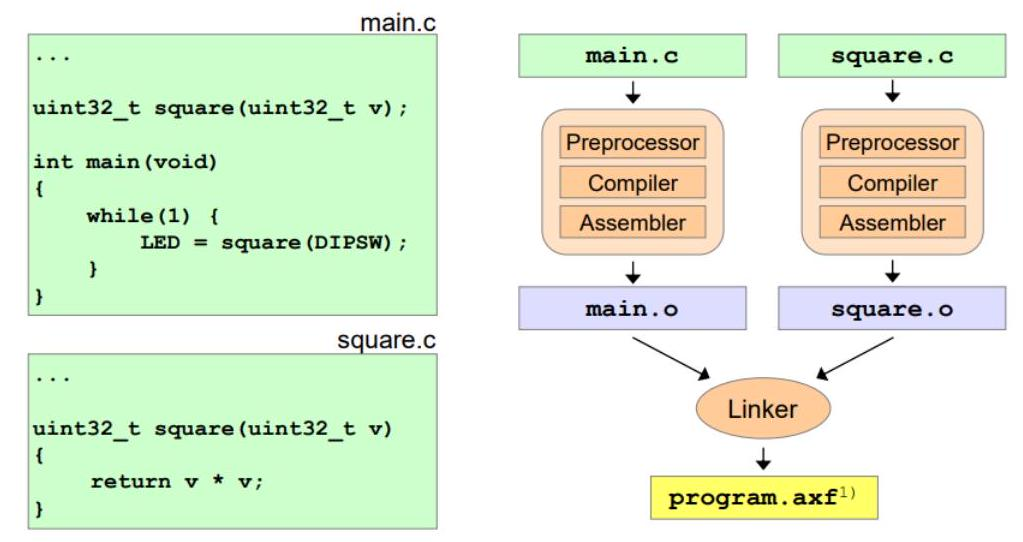
\includegraphics[width=\linewidth]{images/2024_12_29_79e6b22f503fb7b4f718g-10(2)}
\end{definition}

\begin{concept}{Tool Chain Components}
Essential tools for development:

\begin{minipage}[t]{0.5\textwidth}
  \begin{itemize}
    \item \textbf{Compiler (armcc)}:
      \begin{itemize}
        \item Translates C to assembly
        \item Performs optimizations
        \item Generates object files
      \end{itemize}
    \item \textbf{Assembler (armasm)}:
      \begin{itemize}
        \item Processes assembly code
        \item Creates object files
        \item Handles directives
      \end{itemize}
  \end{itemize}
\end{minipage}
\begin{minipage}[t]{0.5\textwidth}
  \begin{itemize}
    \item \textbf{Linker (armlink)}:
      \begin{itemize}
        \item Combines object files
        \item Resolves references
        \item Creates executable
      \end{itemize}
    \item \textbf{Library Manager (armar)}:
      \begin{itemize}
        \item Creates/maintains libraries
        \item Adds/removes object files
        \item Archives multiple objects
      \end{itemize}
  \end{itemize}
\end{minipage}
\end{concept}

\begin{theorem}{Guidelines for Modular Programming}
Key design principles:
\begin{itemize}
  \item \textbf{High Cohesion}: Group related functionality together
    \begin{itemize}
      \item Each module fulfills a single defined task
      \item Lean external interface
    \end{itemize}
  \item \textbf{Low Coupling}: Minimize dependencies between modules
    \begin{itemize}
      \item Clear and minimal interfaces
      \item Easy to modify individual modules
    \end{itemize}
  \item \textbf{Information Hiding}: Split interface from implementation
    \begin{itemize}
      \item Don't expose unnecessary details
      \item Maintain freedom to change internals
    \end{itemize}
\end{itemize}
\end{theorem}

\begin{corollary}{Benefits of Modular Programming}
Key advantages:

\textbf{Team Development}: Multiple developers working on same codebase
    \begin{itemize}
      \item Clear ownership of modules
    \end{itemize}
\textbf{Code Organization}: Logical partitioning/grouping of functionality
    \begin{itemize}
      \item Easier code reuse an better maintainability/understandability
    \end{itemize}
\textbf{Development Efficiency}:
    \begin{itemize}
      \item Individual module testing
      \item Faster compilation (only recompile changed modules)
      \item Reusable library creation
    \end{itemize}
\textbf{Language Integration}: Mix C and assembly modules
    \begin{itemize}
      \item Language-specific optimizations (best of both worlds)
    \end{itemize}
\end{corollary}

\begin{remark}
Important considerations:
\begin{itemize}
  \item Use consistent naming conventions
  \item Document module interfaces clearly
  \item Consider initialization dependencies
  \item Test modules independently
  \item Maintain version control
  \item Document build requirements
\end{itemize}
\end{remark}





\begin{definition}{Module Linkage}
Keywords for controlling module interfaces:
\begin{itemize}
  \item \textbf{EXPORT}: Make symbol available to other modules
  \item \textbf{IMPORT}: Use symbol from another module
  \item Internal symbols: Neither IMPORT nor EXPORT
\end{itemize}

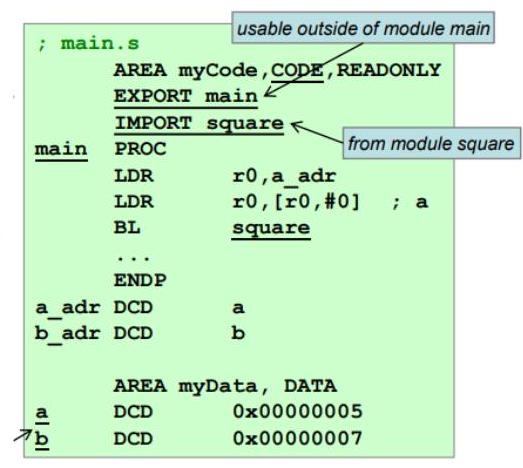
\includegraphics[width=0.7\linewidth]{images/2024_12_29_79e6b22f503fb7b4f718g-10(1)}
\end{definition}

\begin{example2}{Module Interface Example}
\begin{lstlisting}[language=armasm, style=basesmol]
    ; Module A - Defining function
    AREA myCode, CODE, READONLY
    EXPORT myFunction    ; Make available externally
myFunction
    PUSH    {LR}
    ; function code here
    POP     {PC}
    
    ; Module B - Using function
    AREA myCode, CODE, READONLY
    IMPORT myFunction    ; Use external function
    
    BL      myFunction   ; Call the function
\end{lstlisting}
\end{example2}


\begin{formula}{Linkage Types in C}
Three types of linkage:

\textbf{External Linkage}:
    \begin{itemize}
      \item Global names available to all modules
      \item Default for functions and global variables
\begin{lstlisting}[language=C, style=basesmol]
int global_var;           // External linkage
void global_func(void);   // External linkage
\end{lstlisting}
    \end{itemize}
\textbf{Internal Linkage}:
    \begin{itemize}
      \item Names only available within module
      \item Created using 'static' keyword
\begin{lstlisting}[language=C, style=basesmol]
static int module_var;    // Internal linkage
static void local_func(void); // Internal linkage
\end{lstlisting}
    \end{itemize}
\textbf{No Linkage}:
    \begin{itemize}
      \item Local variables and function parameters
      \item Scope limited to block
\begin{lstlisting}[language=C, style=basesmol]
void func(void) {
    int local_var;       // No linkage
    static int static_var; // Internal linkage
}
\end{lstlisting}
    \end{itemize}
\end{formula}
%TODO: add linkage types in assembly




\begin{definition}{Linker Input - Object Files}
\begin{itemize}
  \item \textbf{Code Section}: Based at address 0x0
    \begin{itemize}
      \item Program code and constant data (READONLY) of the module
    \end{itemize}
  \item \textbf{Data Section}: Based at address 0x0
    \begin{itemize}
      \item all global variables and initialized data
    \end{itemize}
  \item \textbf{Symbol Table}: References to external symbols
    \begin{itemize}
      \item All symbols with their attributes like global/local status
    \end{itemize}
  \item \textbf{Relocation Table}: Instructions for adjusting addresses:
    \begin{itemize}
      \item which bytes of the data and code sections need to be modified (and how) after merging the sections in the linking process
      \item Applied during linking process
    \end{itemize}
\end{itemize}
ARM tool chain uses ELF (Executable and Linkable Format) for object files.
\end{definition}

\begin{example2}{Object File Structure}
  File sections:
\begin{lstlisting}[language=armasm, style=basesmol]
; 1. '.text' section (Code):
0x00000000: 4604  MOV     r4,r0
0x00000002: 0040  LSLS    r0,r0,#1
0x00000004: 4420  ADD     r0,r4
; 2. '.data' section:
0x00000000: Initial values for global data
; 3. Symbol table:
; #  Name      Value   Type   Binding
  6  myFunc    0x0000  CODE   Global
  7  extVar    0x0000  DATA   Reference
; 4. Relocation entries:
Offset   Type         Symbol
0x0006   R_ARM_REL32  extVar
\end{lstlisting}
\end{example2}

\begin{concept}{Linker Operation}\\
\textbf{Linker tasks:}
\begin{itemize}
  \item Merge object file code sections
  \item Merge object file data sections
  \item Symbol Resolution: Resolve symbol references between modules
  \item Address relocation: Relocate addresses to final positions
\end{itemize}

\textbf{Linker output:} AXF = ARM executable file

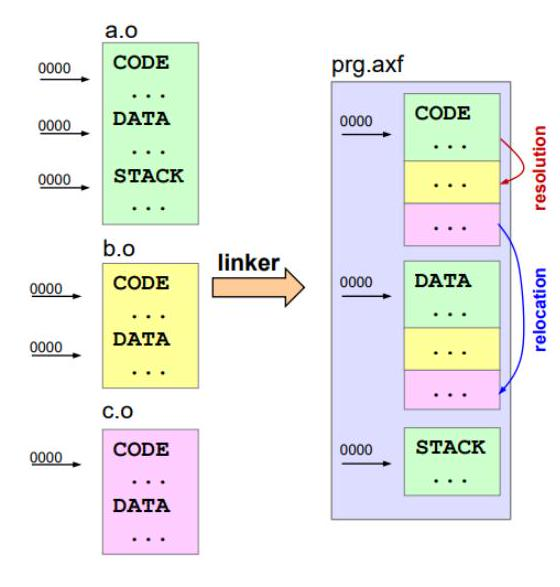
\includegraphics[width=0.8\linewidth]{images/2024_12_29_79e6b22f503fb7b4f718g-10}
\end{concept}

\begin{KR}{Symbol Resolution and Relocation}
Steps in linking process:

1. Symbol Resolution:
\begin{lstlisting}[language=armasm, style=basesmol]
    ; In module1.s
    AREA |.text|, CODE, READONLY
    EXPORT func1
func1
    ; function code
    
    ; In module2.s
    AREA |.text|, CODE, READONLY
    IMPORT func1
    BL      func1    ; Reference to resolve
\end{lstlisting}

2. Relocation:
\begin{lstlisting}[language=armasm, style=basesmol]
    ; Before relocation
    BL      func1    ; Relative offset
    
    ; After relocation
    BL      0x08000234  ; Absolute address
\end{lstlisting}
\end{KR}

\begin{KR}{Creating Modular Programs}
Steps for modular development:
\begin{enumerate}
  \item Design module structure:
    \begin{itemize}
      \item Identify clear boundaries
      \item Define interfaces
    \end{itemize}
  \item Create individual modules:
    \begin{itemize}
      \item Declare IMPORT/EXPORT
      \item Implement functionality
    \end{itemize}
  \item Compile modules separately
  \item Link modules:
    \begin{itemize}
      \item Resolve references
      \item Create executable
    \end{itemize}
  \item Test integrated system
\end{enumerate}
\end{KR}

\begin{KR}{Library Creation and Use}
Steps for creating and using libraries:

1. Create library source files:
\begin{lstlisting}[language=C, style=basesmol]
// lib.h
void lib_func(int x);

// lib.c
void lib_func(int x) {
    // Implementation
}
\end{lstlisting}

2. Compile to object files:
\begin{lstlisting}[style=basesmol]
armcc -c lib.c -o lib.o
\end{lstlisting}

3. Create static library:
\begin{lstlisting}[style=basesmol]
armar --create libmy.a lib.o
\end{lstlisting}

4. Link with library:
\begin{lstlisting}[style=basesmol]
armlink main.o libmy.a -o program.axf
\end{lstlisting}
\end{KR}

\begin{example2}{Library Usage Example}
  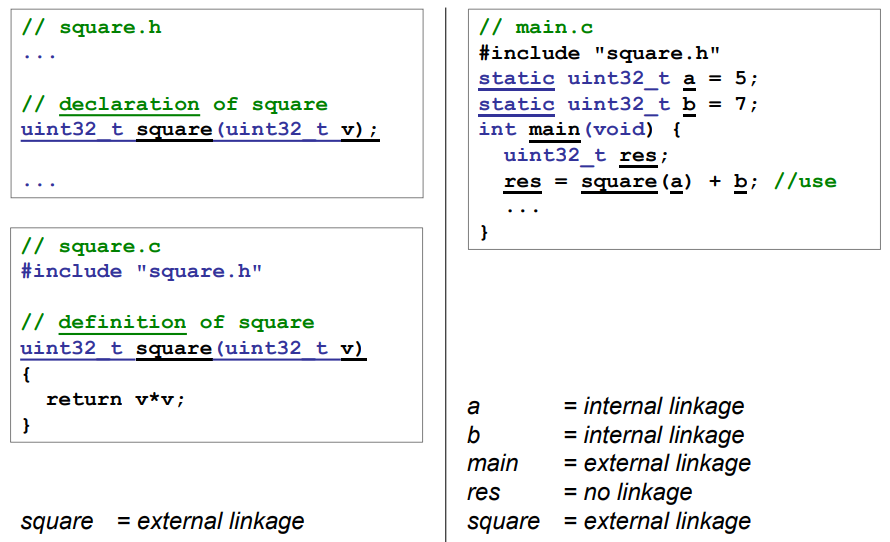
\includegraphics[width=\linewidth]{images/modular_coding_linking_lectureexample.png}
\end{example2}



